\documentclass[doktyp=studarbeit]{TUBAFarbeiten}

\usepackage{selinput}% Auswahl der Dateikodierung (ansi,latin1,utf8,...)
\usepackage[T1]{fontenc}% Einstellung Fontencoding
\usepackage{amsmath}
\usepackage[section]{placeins}
%\usepackage{titlesec}
\usepackage{xcolor}
\usepackage{listings}
% \usepackage{hyperref}
\usepackage{csquotes}% Einstellung zu Anführungszeichen; wird von biblatex.sty gefordert

\newcommand\tab[1][5mm]{\hspace*{#1}}
\newtheorem{thm}{Theorem}
\newtheorem{lem}[thm]{Lemma}
	\SelectInputMappings{adieresis={ä},germandbls={ß},Euro={€}}% Zeichenzuordnung für selinput.sty

% Packages for images and caption in figures
\usepackage{graphicx}
\graphicspath{ {./img/} }
\usepackage{subcaption}

\definecolor{mGreen}{rgb}{0,0.6,0}
\definecolor{mGray}{rgb}{0.5,0.5,0.5}
\definecolor{mPurple}{rgb}{0.58,0,0.82}
\definecolor{backgroundColour}{rgb}{0.95,0.95,0.92}

\lstdefinestyle{CStyle}{
    backgroundcolor=\color{backgroundColour},   
    commentstyle=\color{mGreen},
    keywordstyle=\color{magenta},
    numberstyle=\tiny\color{mGray},
    stringstyle=\color{mPurple},
    basicstyle=\footnotesize,
    breakatwhitespace=false,         
    breaklines=true,                 
    captionpos=b,                    
    keepspaces=true,                 
    numbers=left,                    
    numbersep=5pt,                  
    showspaces=false,                
    showstringspaces=false,
    showtabs=false,                  
    tabsize=2,
    language=C
}

\usepackage[backend=biber,sortlocale=de_DE_phonebook]{biblatex}
\addbibresource{references.bib}

%\usepackage{setspace}% Einstellungen Zeilenabstand
	%\onehalfspacing% Einstellungen Zeilenabstand

\TUBAFFakultaet{Fakultät für Mathematik und Informatik}
\TUBAFInstitut{Institut für Informatik}

\TUBAFTitel[OpenGL Game: Achtung, die Kurve!]{OpenGL Game: Achtung, die Kurve!}
\TUBAFBetreuer{M.Sc. Jonas Treumer}
\TUBAFKorrektor{M.Sc. Ben Lorenz}
\TUBAFAutor[Al Nomer/Valdés]{Simon Al Nomer\newline Hernán Felipe Valdés González}
\TUBAFStudiengang{Bachelor Angewandte Informatik}
\TUBAFMatrikel{64\,082\newline 63\,952}
\TUBAFDatum[2020-10-19]{19. Oktober 2020}

\begin{document}

\maketitle

\TUBAFErklaerungsseite

%%%%%%%%%%%%%%%%%%%%%%%%%%%%%%%%%%%%%%%%%%%%%%%%%%%%%%%%%%%%%%%%%%%%%%%%%%%%%%%%%%%%%%%%%%%%%%%%%%%%%%%
\addsec{Zusammenfassung}% wird die KLassenoption kapitel=true gewählt, so muß hier \addchap{Zusammenfassung} stehen
Implementierung des Spieles ''Achtung, die Kurve'' in C++ mit OpenGL für die 
Lehreveranstaltung ''Multimedia''.

%%%%%%%%%%%%%%%%%%%%%%%%%%%%%%%%%%%%%%%%%%%%%%%%%%%%%%%%%%%%%%%%%%%%%%%%%%%%%%%%%%%%%%%%%%%%%%%%%%%%%%%%


\KOMAoptions{
	listof=totoc	% Abbildungs- und Tabellenverzeichnis im Inhaltsverzeichnis
}

\tableofcontents
\listoffigures
\listoftables

\newpage

\section{Einführung}

Achtung, Die Kurve ist ein Multiplayer-Spiel, welches im Jahr 1995 von 
Filip Oščádal und Kamil Doležal in DOS entwickelt wurde. Im Jahr 2010 wurde 
eine neue Version des Spiels unter dem Namen “Achtung, die Kurve! Flash Remake”
veröffentlicht. Diese Version ist mit Adobe Flash von Geert van den Burg 
entwickelt worden und kann online gespielt werden.

Nachdem das Spiel großen Zuspruch fand, beschloss van den Burg, sich mit 
Robin Brouns zusammenzuschließen und eine Fortsetzung zu entwickeln, welche 
2011 unter den Namen Curve Fever (Originaltitel “Achtung, die Kurve! 2”) 
veröffentlicht wurde und online gespielt werden kann.

In den folgenden Jahren wurden dem Spiel immer weiter neue Features 
hinzugefügt wie zum Beispiel verschiedene Boni, die Möglichkeit, in einem Team 
zu spielen, oder das Bestehen einer Rangliste.

2015 sammelte van den Burg ein Team um sich, um eine neue Version des Spiels in 
HTML5 zu implementieren, welche im September 2016 auf den Markt kam.

\begin{figure}[!h]
	\centering
	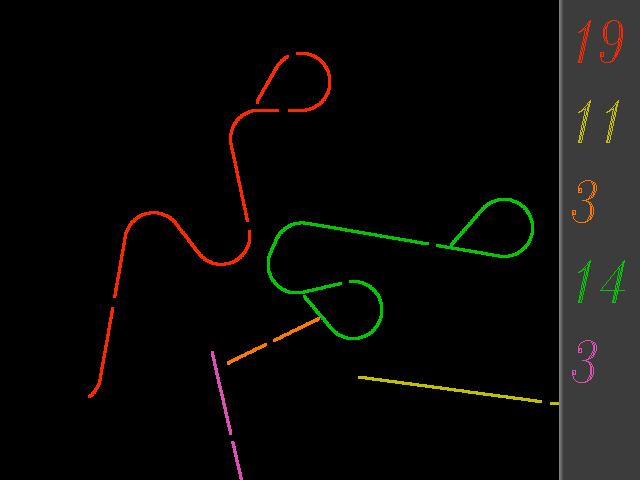
\includegraphics[width=0.7\linewidth]{dos-version.png}
	\caption{Original DOS Version von Achtung, die Kurve! (1995)}
	\label{fig:dos-version}
\end{figure}

\begin{figure}[!h]
	\centering
	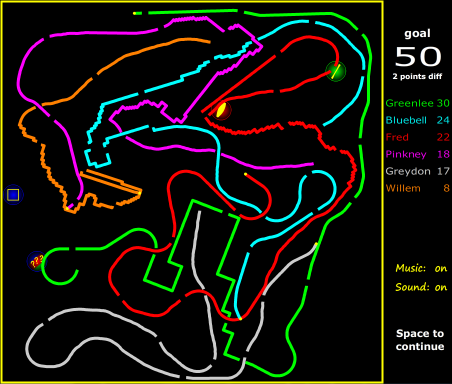
\includegraphics[width=0.7\linewidth]{flash-version.png}
	\caption{Flash remake von Achtung, die Kurve! (2010)}
	\label{fig:flash-version}
\end{figure}

Die Implementierung unseres Spiels basiert auf die Version von 1995 in 
Kombination mit dem Stil der Flash Version.

\subsection{Spielmechanik}

Im Spiel können bis zu 6 Spieler zusammen mit einem Bildschirm und einer 
Tastatur spielen. Jeder Spieler besitzt zwei vorbestimmten Tasten, die rechts 
und links symbolisieren. Um das Spiel zu starten, müssen mindestens 
2 Spieler spielen.  Der Ziel vom Spiel ist, dass der Spieler am Leben 
solange wie möglich bleibt.

Jeder Spieler wird mit einem Kreis dargestellt, der mit jeder Bewegung einen 
Pfad mit der Farbe des Spielers hinterlässt. Der Spieler darf nur nach rechts 
und links die Richtung seiner Bewegung ändern. Wenn der Spieler nicht reagiert, 
wird er weiter in der alten Richtung sich bewegen.

Ein Spieler verliert, wenn er gegen seine eigene Linie, die Linie anderen 
Spieler,  oder den Rand gestoßen hat. Das Spiel ist zu Ende wenn nur ein 
Spieler noch am Leben ist.

\section{Softwaredokumentation}

Unseres Projekt hat als basis den Code, der zusammen während der Vorlesung 
erstellt wurde, genommen und in C++ migriert. 
Die Entscheidung, um das Spiel in C++ statt C zu programmieren, lag 
insbesondere wegen der Standardbibliotheken von C++ und deren implementierten 
Daten Strukturen sowie die Eigenschaft mit Klassen zu programmieren.

\subsection{GameState}

\begin{figure}
    \centering
    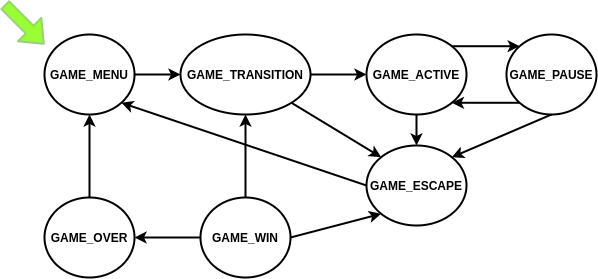
\includegraphics[width=0.7\linewidth]{state_machine.png}
	\caption{Darstellung unseren Zustandsautomat}
	\label{fig:state-machine}
\end{figure}


\printbibliography[heading=bibintoc]
\end{document}